\PassOptionsToPackage{unicode=true}{hyperref} % options for packages loaded elsewhere
\PassOptionsToPackage{hyphens}{url}
%
\documentclass[]{book}
\usepackage{lmodern}
\usepackage{amssymb,amsmath}
\usepackage{ifxetex,ifluatex}
\usepackage{fixltx2e} % provides \textsubscript
\ifnum 0\ifxetex 1\fi\ifluatex 1\fi=0 % if pdftex
  \usepackage[T1]{fontenc}
  \usepackage[utf8]{inputenc}
  \usepackage{textcomp} % provides euro and other symbols
\else % if luatex or xelatex
  \usepackage{unicode-math}
  \defaultfontfeatures{Ligatures=TeX,Scale=MatchLowercase}
\fi
% use upquote if available, for straight quotes in verbatim environments
\IfFileExists{upquote.sty}{\usepackage{upquote}}{}
% use microtype if available
\IfFileExists{microtype.sty}{%
\usepackage[]{microtype}
\UseMicrotypeSet[protrusion]{basicmath} % disable protrusion for tt fonts
}{}
\IfFileExists{parskip.sty}{%
\usepackage{parskip}
}{% else
\setlength{\parindent}{0pt}
\setlength{\parskip}{6pt plus 2pt minus 1pt}
}
\usepackage{hyperref}
\hypersetup{
            pdftitle={Term project draft},
            pdfauthor={Kipling Klimas},
            pdfborder={0 0 0},
            breaklinks=true}
\urlstyle{same}  % don't use monospace font for urls
\usepackage{color}
\usepackage{fancyvrb}
\newcommand{\VerbBar}{|}
\newcommand{\VERB}{\Verb[commandchars=\\\{\}]}
\DefineVerbatimEnvironment{Highlighting}{Verbatim}{commandchars=\\\{\}}
% Add ',fontsize=\small' for more characters per line
\usepackage{framed}
\definecolor{shadecolor}{RGB}{248,248,248}
\newenvironment{Shaded}{\begin{snugshade}}{\end{snugshade}}
\newcommand{\AlertTok}[1]{\textcolor[rgb]{0.94,0.16,0.16}{#1}}
\newcommand{\AnnotationTok}[1]{\textcolor[rgb]{0.56,0.35,0.01}{\textbf{\textit{#1}}}}
\newcommand{\AttributeTok}[1]{\textcolor[rgb]{0.77,0.63,0.00}{#1}}
\newcommand{\BaseNTok}[1]{\textcolor[rgb]{0.00,0.00,0.81}{#1}}
\newcommand{\BuiltInTok}[1]{#1}
\newcommand{\CharTok}[1]{\textcolor[rgb]{0.31,0.60,0.02}{#1}}
\newcommand{\CommentTok}[1]{\textcolor[rgb]{0.56,0.35,0.01}{\textit{#1}}}
\newcommand{\CommentVarTok}[1]{\textcolor[rgb]{0.56,0.35,0.01}{\textbf{\textit{#1}}}}
\newcommand{\ConstantTok}[1]{\textcolor[rgb]{0.00,0.00,0.00}{#1}}
\newcommand{\ControlFlowTok}[1]{\textcolor[rgb]{0.13,0.29,0.53}{\textbf{#1}}}
\newcommand{\DataTypeTok}[1]{\textcolor[rgb]{0.13,0.29,0.53}{#1}}
\newcommand{\DecValTok}[1]{\textcolor[rgb]{0.00,0.00,0.81}{#1}}
\newcommand{\DocumentationTok}[1]{\textcolor[rgb]{0.56,0.35,0.01}{\textbf{\textit{#1}}}}
\newcommand{\ErrorTok}[1]{\textcolor[rgb]{0.64,0.00,0.00}{\textbf{#1}}}
\newcommand{\ExtensionTok}[1]{#1}
\newcommand{\FloatTok}[1]{\textcolor[rgb]{0.00,0.00,0.81}{#1}}
\newcommand{\FunctionTok}[1]{\textcolor[rgb]{0.00,0.00,0.00}{#1}}
\newcommand{\ImportTok}[1]{#1}
\newcommand{\InformationTok}[1]{\textcolor[rgb]{0.56,0.35,0.01}{\textbf{\textit{#1}}}}
\newcommand{\KeywordTok}[1]{\textcolor[rgb]{0.13,0.29,0.53}{\textbf{#1}}}
\newcommand{\NormalTok}[1]{#1}
\newcommand{\OperatorTok}[1]{\textcolor[rgb]{0.81,0.36,0.00}{\textbf{#1}}}
\newcommand{\OtherTok}[1]{\textcolor[rgb]{0.56,0.35,0.01}{#1}}
\newcommand{\PreprocessorTok}[1]{\textcolor[rgb]{0.56,0.35,0.01}{\textit{#1}}}
\newcommand{\RegionMarkerTok}[1]{#1}
\newcommand{\SpecialCharTok}[1]{\textcolor[rgb]{0.00,0.00,0.00}{#1}}
\newcommand{\SpecialStringTok}[1]{\textcolor[rgb]{0.31,0.60,0.02}{#1}}
\newcommand{\StringTok}[1]{\textcolor[rgb]{0.31,0.60,0.02}{#1}}
\newcommand{\VariableTok}[1]{\textcolor[rgb]{0.00,0.00,0.00}{#1}}
\newcommand{\VerbatimStringTok}[1]{\textcolor[rgb]{0.31,0.60,0.02}{#1}}
\newcommand{\WarningTok}[1]{\textcolor[rgb]{0.56,0.35,0.01}{\textbf{\textit{#1}}}}
\usepackage{longtable,booktabs}
% Fix footnotes in tables (requires footnote package)
\IfFileExists{footnote.sty}{\usepackage{footnote}\makesavenoteenv{longtable}}{}
\usepackage{graphicx,grffile}
\makeatletter
\def\maxwidth{\ifdim\Gin@nat@width>\linewidth\linewidth\else\Gin@nat@width\fi}
\def\maxheight{\ifdim\Gin@nat@height>\textheight\textheight\else\Gin@nat@height\fi}
\makeatother
% Scale images if necessary, so that they will not overflow the page
% margins by default, and it is still possible to overwrite the defaults
% using explicit options in \includegraphics[width, height, ...]{}
\setkeys{Gin}{width=\maxwidth,height=\maxheight,keepaspectratio}
\setlength{\emergencystretch}{3em}  % prevent overfull lines
\providecommand{\tightlist}{%
  \setlength{\itemsep}{0pt}\setlength{\parskip}{0pt}}
\setcounter{secnumdepth}{5}
% Redefines (sub)paragraphs to behave more like sections
\ifx\paragraph\undefined\else
\let\oldparagraph\paragraph
\renewcommand{\paragraph}[1]{\oldparagraph{#1}\mbox{}}
\fi
\ifx\subparagraph\undefined\else
\let\oldsubparagraph\subparagraph
\renewcommand{\subparagraph}[1]{\oldsubparagraph{#1}\mbox{}}
\fi

% set default figure placement to htbp
\makeatletter
\def\fps@figure{htbp}
\makeatother

\usepackage{booktabs}
\usepackage[]{natbib}
\bibliographystyle{apalike}

\title{Term project draft}
\author{Kipling Klimas}
\date{2021-04-27}

\begin{document}
\maketitle

{
\setcounter{tocdepth}{1}
\tableofcontents
}
\hypertarget{introduction}{%
\chapter{Introduction}\label{introduction}}

Wildfires can have significant impacts on both ecosystems and human assets in forested environments.

In the fire-prone mixed conifer/aspen forests of the Intermountain West (IW) fuel reduction treatments including stand thinning, mastication, aspen promotion and prescribed fire are implemented to reduce the risk, incidence and/or extent of destructive, high severity wildfire. Due to the high value of forested resources in the IW and the risk of post-fire sediment transport or debris flows downstream from burned areas, fuel reduction treatments are important landscape-scale tools that forest managers use to protect forest assets. However, the complex and pyrophytic nature of IW forests, along environmental and societal constraints, lends to barriers against spatially targeted implementation of fuel reduction treatments in high-value forested watersheds (Larson \& Churchill, 2012).

Modeling the effect of fuel reduction treatments on fire behavior in fire-prone forests of the western United States has shown that targeted fuel reduction treatments are more effective at altering fire behavior (i.e.~rate of spread, flame length) than randomly or indiscriminately applied treatments (Kim et al., 2009; Minas et al., 2014; Prichard et al., 2020). The spatial distribution of treatments must then follow a prioritization hierarchy, such as concentrated, dispersed or regularly arranged treated areas within a forest (Kim et al., 2009), but the economic trade-off and efficacy of treatment distribution warrants greater examination in IW forests, where fuel treatments are applied to reduce the risk of high severity wildfire (Barros et al., 2019). By altering fire behavior through landscape-scale treatments, forest managers hope to reduce the extent of high-severity burned areas and mitigate downstream consequences of high-severity wildfire, such as the development of debris flows which can have negative impacts on high value assets such as reservoirs or fish habitat.

\hypertarget{data}{%
\chapter{Data description and database structure}\label{data}}

Forest strcuture and fuels data are needed to model fire behavior and predict burn severity spatially.

\begin{center}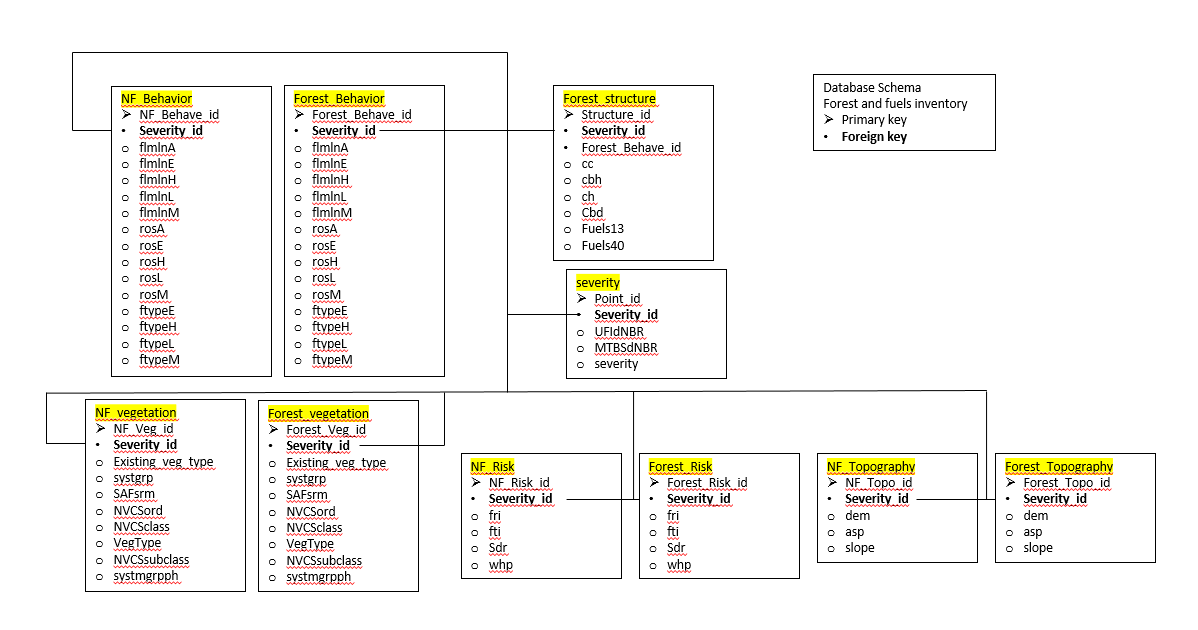
\includegraphics{db_structure} \end{center}

Figure 1: databse structure for forest and fuels inventory.

This database structure is compatible with tree and stand level forest simulation software such as the Forest Vegetation Simulator (FVS) which can be used to model forest structure over time. An advantage of this approach and structure is these data allow detailed simulation of mortality during fire.

Tree level data are related to plot polygons that allow for stand-level simulation. Fuels data is required for modeled fire behavior, such as flame length, rate or spread or fire type (surface, passive or active).

Whether or not these tables become populated remains to be seen- a disadvantage of this approach is that fuel reduction treatments are not readily applied to the landscape in question. It is also only useable for fire behavior modeling as an ArcMap toolbar extension.

\hypertarget{creation}{%
\chapter{Database creation}\label{creation}}

Start

Install and open packages \texttt{RSQLite}

\begin{Shaded}
\begin{Highlighting}[]
\KeywordTok{install.packages}\NormalTok{(}\StringTok{"RSQLite"}\NormalTok{)}
\KeywordTok{library}\NormalTok{(RSQLite)}
\end{Highlighting}
\end{Shaded}

Establish database connection

Connecting to the term\_project database

\begin{Shaded}
\begin{Highlighting}[]
\NormalTok{term_project <-}\StringTok{ }\KeywordTok{dbConnect}\NormalTok{(}\DataTypeTok{drv =}\NormalTok{ RSQLite}\OperatorTok{::}\KeywordTok{SQLite}\NormalTok{(),}
                        \StringTok{"C:/Users/A02345823/Box/Lab_Group/Kipling/Classes/WILD6900_EcoRepSci/Term_project/Term_project/database/severity.db"}\NormalTok{)}
\end{Highlighting}
\end{Shaded}

Create severity table
Term project database creation based on structure in figure 1

\begin{Shaded}
\begin{Highlighting}[]
\KeywordTok{dbExecute}\NormalTok{(term_project, }\StringTok{"CREATE TABLE severity(}
\StringTok{severity_id integer NOT NULL PRIMARY KEY,}
\StringTok{MTBSdNBR float,}
\StringTok{severity float}
\StringTok{);"}\NormalTok{)}
\end{Highlighting}
\end{Shaded}

Create forest behavior table

\begin{Shaded}
\begin{Highlighting}[]
\KeywordTok{dbExecute}\NormalTok{(term_project, }\StringTok{"CREATE TABLE forest_behavior(}
\StringTok{forest_behave_id integer NOT NULL PRIMARY KEY,}
\StringTok{severity_id float,}
\StringTok{flmlnA float,}
\StringTok{flmlnE float,}
\StringTok{flmlnH float,}
\StringTok{flmlnL float,}
\StringTok{flmlnM float,}
\StringTok{ftype_E float,}
\StringTok{ftype_H float,}
\StringTok{ftype_L float,}
\StringTok{ftype_M float,}
\StringTok{ros float,}
\StringTok{rosE float,}
\StringTok{rosH float,}
\StringTok{rosL float,}
\StringTok{rosM float,}
\StringTok{FOREIGN KEY(severity_id) REFERENCES severity(severity_id)}
\StringTok{);"}\NormalTok{)}
\end{Highlighting}
\end{Shaded}

Create forest risk table

\begin{Shaded}
\begin{Highlighting}[]
\KeywordTok{dbExecute}\NormalTok{(term_project, }\StringTok{"CREATE TABLE forest_risk(}
\StringTok{forest_risk_id integer NOT NULL PRIMARY KEY,}
\StringTok{severity_id float,}
\StringTok{fri float,}
\StringTok{fti float,}
\StringTok{sdr varchar(12),}
\StringTok{WHP float,}
\StringTok{FOREIGN KEY(severity_id) REFERENCES severity(severity_id)}
\StringTok{);"}\NormalTok{)}
\end{Highlighting}
\end{Shaded}

Create forest\_structure table

\begin{Shaded}
\begin{Highlighting}[]
\KeywordTok{dbExecute}\NormalTok{(term_project, }\StringTok{"CREATE TABLE forest_structure(}
\StringTok{str_id integer NOT NULL PRIMARY KEY,}
\StringTok{severity_id float,}
\StringTok{wwacbd float,}
\StringTok{wwacbh float,}
\StringTok{wwacc float,}
\StringTok{wwach float,}
\StringTok{wwafuel13 float,}
\StringTok{wwafuel40 float,}
\StringTok{FOREIGN KEY(severity_id) REFERENCES severity(severity_id)}
\StringTok{);"}\NormalTok{)}
\end{Highlighting}
\end{Shaded}

Create forest\_topo table

\begin{Shaded}
\begin{Highlighting}[]
\KeywordTok{dbExecute}\NormalTok{(term_project, }\StringTok{"CREATE TABLE forest_topo(}
\StringTok{forest_topo_id integer NOT NULL PRIMARY KEY,}
\StringTok{severity_id float,}
\StringTok{asp varchar(5),}
\StringTok{dem float,}
\StringTok{slope float,}
\StringTok{FOREIGN KEY(severity_id) REFERENCES severity(severity_id)}
\StringTok{);"}\NormalTok{)}
\end{Highlighting}
\end{Shaded}

Create forest\_veg table

\begin{Shaded}
\begin{Highlighting}[]
\KeywordTok{dbExecute}\NormalTok{(term_project, }\StringTok{"CREATE TABLE forest_veg(}
\StringTok{forest_veg_id integer NOT NULL PRIMARY KEY,}
\StringTok{severity_id float,}
\StringTok{EVT varchar(60),}
\StringTok{SystGrp varchar(60),}
\StringTok{SAFSrm varchar(60),}
\StringTok{NVCSOrd varchar(16),}
\StringTok{NVCSclass varchar(25),}
\StringTok{NVCSsubclass varchar(40),}
\StringTok{SYSTMGRPPH varchar(30),}
\StringTok{FOREIGN KEY(severity_id) REFERENCES severity(severity_id)}
\StringTok{);"}\NormalTok{)}
\end{Highlighting}
\end{Shaded}

Create non-forest db tables

Create non-forest behavior table

\begin{Shaded}
\begin{Highlighting}[]
\KeywordTok{dbExecute}\NormalTok{(term_project, }\StringTok{"CREATE TABLE nf_behavior(}
\StringTok{nf_behave_id integer NOT NULL PRIMARY KEY,}
\StringTok{severity_id float,}
\StringTok{flmlnA float,}
\StringTok{flmlnE float,}
\StringTok{flmlnH float,}
\StringTok{flmlnL float,}
\StringTok{flmlnM float,}
\StringTok{ftype_E float,}
\StringTok{ftype_H float,}
\StringTok{ftype_L float,}
\StringTok{ftype_M float,}
\StringTok{ros float,}
\StringTok{rosE float,}
\StringTok{rosH float,}
\StringTok{rosL float,}
\StringTok{rosM float,}
\StringTok{FOREIGN KEY(severity_id) REFERENCES severity(severity_id)}
\StringTok{);"}\NormalTok{)}
\end{Highlighting}
\end{Shaded}

Create non-forest risk table

\begin{Shaded}
\begin{Highlighting}[]
\KeywordTok{dbExecute}\NormalTok{(term_project, }\StringTok{"CREATE TABLE nf_risk(}
\StringTok{nf_risk_id integer NOT NULL PRIMARY KEY,}
\StringTok{severity_id float,}
\StringTok{fri float,}
\StringTok{fti float,}
\StringTok{sdr varchar(12),}
\StringTok{WHP float,}
\StringTok{FOREIGN KEY(severity_id) REFERENCES severity(severity_id)}
\StringTok{);"}\NormalTok{)}
\end{Highlighting}
\end{Shaded}

Create non-forest\_structure table

\begin{Shaded}
\begin{Highlighting}[]
\KeywordTok{dbExecute}\NormalTok{(term_project, }\StringTok{"CREATE TABLE nf_structure(}
\StringTok{nf_str_id integer NOT NULL PRIMARY KEY,}
\StringTok{severity_id float,}
\StringTok{wwacbd float,}
\StringTok{wwacbh float,}
\StringTok{wwacc float,}
\StringTok{wwach float,}
\StringTok{wwafuel13 float,}
\StringTok{wwafuel40 float,}
\StringTok{FOREIGN KEY(severity_id) REFERENCES severity(severity_id)}
\StringTok{);"}\NormalTok{)}
\end{Highlighting}
\end{Shaded}

Create non-forest\_topo table

\begin{Shaded}
\begin{Highlighting}[]
\KeywordTok{dbExecute}\NormalTok{(term_project, }\StringTok{"CREATE TABLE nf_topo(}
\StringTok{nf_topo_id integer NOT NULL PRIMARY KEY,}
\StringTok{severity_id float,}
\StringTok{asp varchar(5),}
\StringTok{dem float,}
\StringTok{slope float,}
\StringTok{FOREIGN KEY(severity_id) REFERENCES severity(severity_id)}
\StringTok{);"}\NormalTok{)}
\end{Highlighting}
\end{Shaded}

Create non-forest\_veg table

\begin{Shaded}
\begin{Highlighting}[]
\KeywordTok{dbExecute}\NormalTok{(term_project, }\StringTok{"CREATE TABLE nf_veg(}
\StringTok{nf_veg_id integer NOT NULL PRIMARY KEY,}
\StringTok{severity_id float,}
\StringTok{EVT varchar(60),}
\StringTok{SystGrp varchar(60),}
\StringTok{SAFSrm varchar(60),}
\StringTok{NVCSOrd varchar(16),}
\StringTok{NVCSclass varchar(25),}
\StringTok{NVCSsubclass varchar(40),}
\StringTok{SYSTMGRPPH varchar(30),}
\StringTok{FOREIGN KEY(severity_id) REFERENCES severity(severity_id)}
\StringTok{);"}\NormalTok{)}
\end{Highlighting}
\end{Shaded}

\hypertarget{SQL}{%
\chapter{Database connection}\label{SQL}}

Start

Install package \texttt{RSQLite}

\begin{Shaded}
\begin{Highlighting}[]
\KeywordTok{install.packages}\NormalTok{(}\StringTok{"RSQLite"}\NormalTok{)}
\KeywordTok{library}\NormalTok{(RSQLite)}
\end{Highlighting}
\end{Shaded}

Establish datebase connection and create tables

\begin{Shaded}
\begin{Highlighting}[]
\NormalTok{severity_db <-}\StringTok{ }\KeywordTok{dbConnect}\NormalTok{(}\DataTypeTok{drv =}\NormalTok{ RSQLite}\OperatorTok{::}\KeywordTok{SQLite}\NormalTok{(),}
                \StringTok{"/Users/kiplingklimas/Box/Lab_Group/Kipling/Classes/WILD6900_EcoRepSci/Term_project/Term_project/database/severity.db"}\NormalTok{)}

\NormalTok{severity <-}\StringTok{ }\KeywordTok{dbGetQuery}\NormalTok{(severity_db, }\StringTok{"SELECT * FROM severity;"}\NormalTok{)}
\NormalTok{forest_behavior <-}\StringTok{ }\KeywordTok{dbGetQuery}\NormalTok{(severity_db, }\StringTok{"SELECT * FROM forest_behavior;"}\NormalTok{)}
\NormalTok{forest_risk <-}\StringTok{ }\KeywordTok{dbGetQuery}\NormalTok{(severity_db, }\StringTok{"SELECT * FROM forest_risk;"}\NormalTok{)}
\NormalTok{forest_structure <-}\StringTok{ }\KeywordTok{dbGetQuery}\NormalTok{(severity_db, }\StringTok{"SELECT * FROM forest_structure;"}\NormalTok{)}
\NormalTok{forest_topo <-}\StringTok{ }\KeywordTok{dbGetQuery}\NormalTok{(severity_db, }\StringTok{"SELECT * FROM forest_topo;"}\NormalTok{)}
\NormalTok{forest_veg <-}\StringTok{ }\KeywordTok{dbGetQuery}\NormalTok{(severity_db, }\StringTok{"SELECT * FROM forest_veg;"}\NormalTok{)}
\NormalTok{nf_behavior <-}\StringTok{ }\KeywordTok{dbGetQuery}\NormalTok{(severity_db, }\StringTok{"SELECT * FROM nf_behavior;"}\NormalTok{)}
\NormalTok{nf_risk <-}\StringTok{ }\KeywordTok{dbGetQuery}\NormalTok{(severity_db, }\StringTok{"SELECT * FROM nf_risk;"}\NormalTok{)}
\NormalTok{nf_structure <-}\StringTok{ }\KeywordTok{dbGetQuery}\NormalTok{(severity_db, }\StringTok{"SELECT * FROM nf_structure;"}\NormalTok{)}
\NormalTok{nf_topo <-}\StringTok{ }\KeywordTok{dbGetQuery}\NormalTok{(severity_db, }\StringTok{"SELECT * FROM nf_topo;"}\NormalTok{)}
\NormalTok{nf_veg <-}\StringTok{ }\KeywordTok{dbGetQuery}\NormalTok{(severity_db, }\StringTok{"SELECT * FROM nf_veg;"}\NormalTok{)}
\end{Highlighting}
\end{Shaded}

\hypertarget{tidyverse}{%
\chapter{Data visualization}\label{tidyverse}}

Install packages \texttt{tidyverse} and \texttt{viridis}

\begin{Shaded}
\begin{Highlighting}[]
\KeywordTok{library}\NormalTok{(tidyverse)}
\end{Highlighting}
\end{Shaded}

\begin{verbatim}
## -- Attaching packages --------------------------------------- tidyverse 1.3.1 --
\end{verbatim}

\begin{verbatim}
## v ggplot2 3.3.3     v purrr   0.3.4
## v tibble  3.1.1     v dplyr   1.0.5
## v tidyr   1.1.3     v stringr 1.4.0
## v readr   1.4.0     v forcats 0.5.1
\end{verbatim}

\begin{verbatim}
## -- Conflicts ------------------------------------------ tidyverse_conflicts() --
## x dplyr::filter() masks stats::filter()
## x dplyr::lag()    masks stats::lag()
\end{verbatim}

\begin{Shaded}
\begin{Highlighting}[]
\KeywordTok{library}\NormalTok{(viridis)}
\end{Highlighting}
\end{Shaded}

\begin{verbatim}
## Loading required package: viridisLite
\end{verbatim}

\begin{Shaded}
\begin{Highlighting}[]
\KeywordTok{library}\NormalTok{(RSQLite)}
\KeywordTok{library}\NormalTok{(DBI)}
\KeywordTok{library}\NormalTok{(ggridges)}
\end{Highlighting}
\end{Shaded}

Connect to database `severity' and create tables

\begin{Shaded}
\begin{Highlighting}[]
\NormalTok{severity_db <-}\StringTok{ }\KeywordTok{dbConnect}\NormalTok{(}\DataTypeTok{drv =}\NormalTok{ RSQLite}\OperatorTok{::}\KeywordTok{SQLite}\NormalTok{(),}
                \StringTok{"/Users/kiplingklimas/Box/Lab_Group/Kipling/Classes/WILD6900_EcoRepSci/Term_project/Term_project/database/severity.db"}\NormalTok{)}

\NormalTok{severity <-}\StringTok{ }\KeywordTok{dbGetQuery}\NormalTok{(severity_db, }\StringTok{"SELECT * FROM severity;"}\NormalTok{)}
\NormalTok{forest_behavior <-}\StringTok{ }\KeywordTok{dbGetQuery}\NormalTok{(severity_db, }\StringTok{"SELECT * FROM forest_behavior;"}\NormalTok{)}
\NormalTok{forest_risk <-}\StringTok{ }\KeywordTok{dbGetQuery}\NormalTok{(severity_db, }\StringTok{"SELECT * FROM forest_risk;"}\NormalTok{)}
\NormalTok{forest_structure <-}\StringTok{ }\KeywordTok{dbGetQuery}\NormalTok{(severity_db, }\StringTok{"SELECT * FROM forest_structure;"}\NormalTok{)}
\NormalTok{forest_topo <-}\StringTok{ }\KeywordTok{dbGetQuery}\NormalTok{(severity_db, }\StringTok{"SELECT * FROM forest_topo;"}\NormalTok{)}
\NormalTok{forest_veg <-}\StringTok{ }\KeywordTok{dbGetQuery}\NormalTok{(severity_db, }\StringTok{"SELECT * FROM forest_veg;"}\NormalTok{)}
\NormalTok{nf_behavior <-}\StringTok{ }\KeywordTok{dbGetQuery}\NormalTok{(severity_db, }\StringTok{"SELECT * FROM nf_behavior;"}\NormalTok{)}
\NormalTok{nf_risk <-}\StringTok{ }\KeywordTok{dbGetQuery}\NormalTok{(severity_db, }\StringTok{"SELECT * FROM nf_risk;"}\NormalTok{)}
\NormalTok{nf_structure <-}\StringTok{ }\KeywordTok{dbGetQuery}\NormalTok{(severity_db, }\StringTok{"SELECT * FROM nf_structure;"}\NormalTok{)}
\NormalTok{nf_topo <-}\StringTok{ }\KeywordTok{dbGetQuery}\NormalTok{(severity_db, }\StringTok{"SELECT * FROM nf_topo;"}\NormalTok{)}
\NormalTok{nf_veg <-}\StringTok{ }\KeywordTok{dbGetQuery}\NormalTok{(severity_db, }\StringTok{"SELECT * FROM nf_veg;"}\NormalTok{)}
\end{Highlighting}
\end{Shaded}

This is fire severity dataset shows the relationship between severity measurements and a variety of predictive variables
including topographic, vegetation, structural and derived risk indices.
Data was differentiated between forest and non-forest points to compare severity relationships between forests and non-forest
landcover systems.

Simple scatter plot of forest severity by elevation (m)

\begin{Shaded}
\begin{Highlighting}[]
\NormalTok{sev <-}\StringTok{ }\NormalTok{forest_topo }\OperatorTok\StringTok{ }
\StringTok{  }\KeywordTok{left_join}\NormalTok{(severity, }\DataTypeTok{by =} \StringTok{"severity_id"}\NormalTok{) }\OperatorTok\StringTok{ }
\StringTok{  }\KeywordTok{select}\NormalTok{(dem, severity)}

\NormalTok{reg <-}\StringTok{ }\KeywordTok{lm}\NormalTok{(}\DataTypeTok{formula=}\NormalTok{ severity }\OperatorTok{~}\StringTok{ }\NormalTok{dem, }\DataTypeTok{data =}\NormalTok{ sev)}
\NormalTok{regs <-}\StringTok{ }\KeywordTok{predict}\NormalTok{(reg, }\DataTypeTok{se.fit =} \OtherTok{TRUE}\NormalTok{)}
\NormalTok{regs <-}\StringTok{ }\KeywordTok{data.frame}\NormalTok{(}\DataTypeTok{mean =}\NormalTok{ regs}\OperatorTok{$}\NormalTok{fit,}
                    \DataTypeTok{upr =}\NormalTok{ regs}\OperatorTok{$}\NormalTok{fit }\OperatorTok{+}\StringTok{ }\FloatTok{1.96} \OperatorTok{*}\StringTok{ }\NormalTok{regs}\OperatorTok{$}\NormalTok{se.fit,}
                    \DataTypeTok{lwr =}\NormalTok{ regs}\OperatorTok{$}\NormalTok{fit }\OperatorTok{-}\StringTok{ }\FloatTok{1.96} \OperatorTok{*}\StringTok{ }\NormalTok{regs}\OperatorTok{$}\NormalTok{se.fit)}
            

\NormalTok{forest_topo }\OperatorTok\StringTok{ }
\StringTok{  }\KeywordTok{left_join}\NormalTok{(severity, }\DataTypeTok{by =} \StringTok{"severity_id"}\NormalTok{) }\OperatorTok\StringTok{ }
\StringTok{  }\KeywordTok{select}\NormalTok{(dem, severity) }\OperatorTok\StringTok{ }
\StringTok{  }\KeywordTok{ggplot}\NormalTok{(}\KeywordTok{aes}\NormalTok{(}\DataTypeTok{x =}\NormalTok{ dem, }\DataTypeTok{y =}\NormalTok{ severity, }\DataTypeTok{color=}\NormalTok{ dem)) }\OperatorTok{+}
\StringTok{  }\KeywordTok{geom_point}\NormalTok{(}\DataTypeTok{alpha =} \FloatTok{0.5}\NormalTok{) }\OperatorTok{+}
\StringTok{  }\KeywordTok{scale_color_viridis_c}\NormalTok{(}\DataTypeTok{option =} \StringTok{"magma"}\NormalTok{) }\OperatorTok{+}
\StringTok{  }\KeywordTok{geom_line}\NormalTok{(}\KeywordTok{aes}\NormalTok{(}\DataTypeTok{y =}\NormalTok{ regs}\OperatorTok{$}\NormalTok{mean, }\DataTypeTok{color =}\NormalTok{ regs}\OperatorTok{$}\NormalTok{mean)) }\OperatorTok{+}
\StringTok{  }\KeywordTok{labs}\NormalTok{(}\DataTypeTok{y =} \StringTok{"Severity (dNBR)"}\NormalTok{, }\DataTypeTok{x =} \StringTok{"Elevation (m)"}\NormalTok{) }\OperatorTok{+}
\StringTok{  }\KeywordTok{theme_light}\NormalTok{() }
\end{Highlighting}
\end{Shaded}

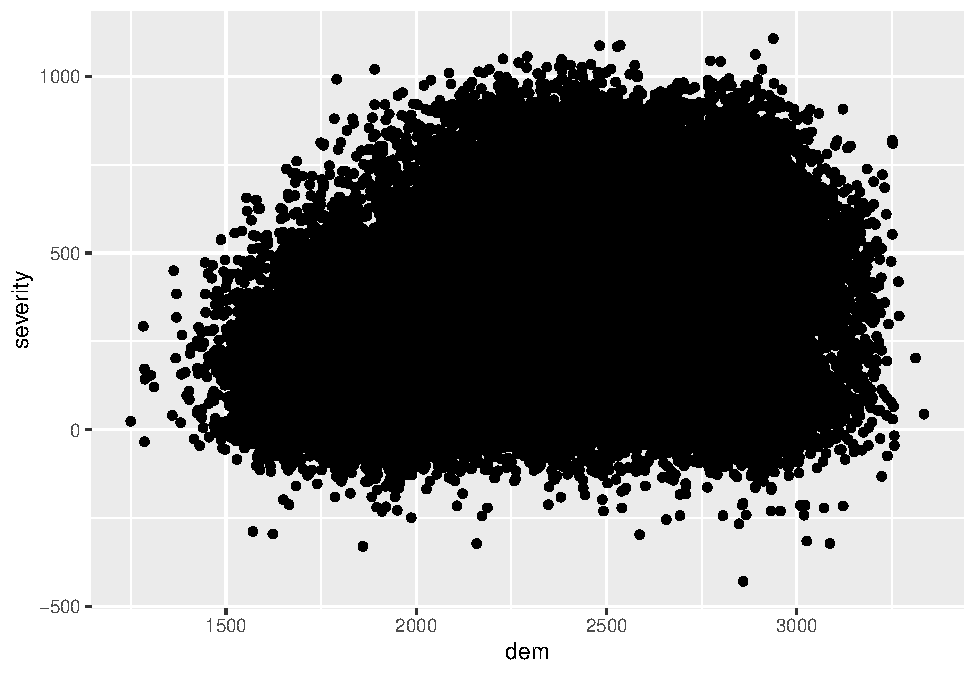
\includegraphics{term_project_files/figure-latex/simple_plots-1.pdf}

Density curves of fire type extreme by severity

\begin{Shaded}
\begin{Highlighting}[]
\NormalTok{forest_behavior }\OperatorTok\StringTok{ }
\StringTok{  }\KeywordTok{left_join}\NormalTok{(severity, }\DataTypeTok{by =} \StringTok{"severity_id"}\NormalTok{) }\OperatorTok\StringTok{ }
\StringTok{  }\KeywordTok{mutate}\NormalTok{(}\DataTypeTok{ftypeE =} \KeywordTok{case_when}\NormalTok{(}
\NormalTok{    ftype_E }\OperatorTok{==}\StringTok{ }\DecValTok{3} \OperatorTok{~}\StringTok{ "Surface"}\NormalTok{,}
\NormalTok{    ftype_E }\OperatorTok{==}\StringTok{ }\DecValTok{4} \OperatorTok{~}\StringTok{ "Passive"}\NormalTok{,}
\NormalTok{    ftype_E }\OperatorTok{==}\StringTok{ }\DecValTok{5} \OperatorTok{~}\StringTok{ "Passive"}\NormalTok{,}
\NormalTok{    ftype_E }\OperatorTok{==}\StringTok{ }\DecValTok{6} \OperatorTok{~}\StringTok{ "Active"}\NormalTok{,}
\NormalTok{    ftype_E }\OperatorTok{==}\StringTok{ }\DecValTok{7} \OperatorTok{~}\StringTok{ "Active"}\NormalTok{,}
\NormalTok{  )) }\OperatorTok\StringTok{ }
\StringTok{  }\KeywordTok{ggplot}\NormalTok{(}\KeywordTok{aes}\NormalTok{(}\DataTypeTok{y =}\NormalTok{ ftypeE, }\DataTypeTok{x =}\NormalTok{ severity, }\DataTypeTok{fill =}\NormalTok{ ftypeE)) }\OperatorTok{+}
\StringTok{  }\NormalTok{ggridges}\OperatorTok{::}\KeywordTok{geom_density_ridges}\NormalTok{(}\DataTypeTok{scale =} \DecValTok{8}\NormalTok{, }\DataTypeTok{alpha =} \FloatTok{0.5}\NormalTok{, }\DataTypeTok{show.legend =} \OtherTok{FALSE}\NormalTok{) }\OperatorTok{+}
\StringTok{  }\KeywordTok{theme}\NormalTok{(}\DataTypeTok{axis.text.x =} \KeywordTok{element_text}\NormalTok{(}\DataTypeTok{angle =} \DecValTok{45}\NormalTok{, }\DataTypeTok{hjust =} \DecValTok{1}\NormalTok{))  }\OperatorTok{+}
\StringTok{  }\KeywordTok{labs}\NormalTok{(}\DataTypeTok{y =} \StringTok{"Density"}\NormalTok{, }\DataTypeTok{x =} \StringTok{"Severity"}\NormalTok{) }\OperatorTok{+}
\StringTok{  }\KeywordTok{scale_color_viridis_d}\NormalTok{(}\DataTypeTok{option =} \StringTok{"magma"}\NormalTok{) }\OperatorTok{+}
\StringTok{  }\KeywordTok{theme_minimal}\NormalTok{()}
\end{Highlighting}
\end{Shaded}

\begin{verbatim}
## Picking joint bandwidth of 29.2
\end{verbatim}

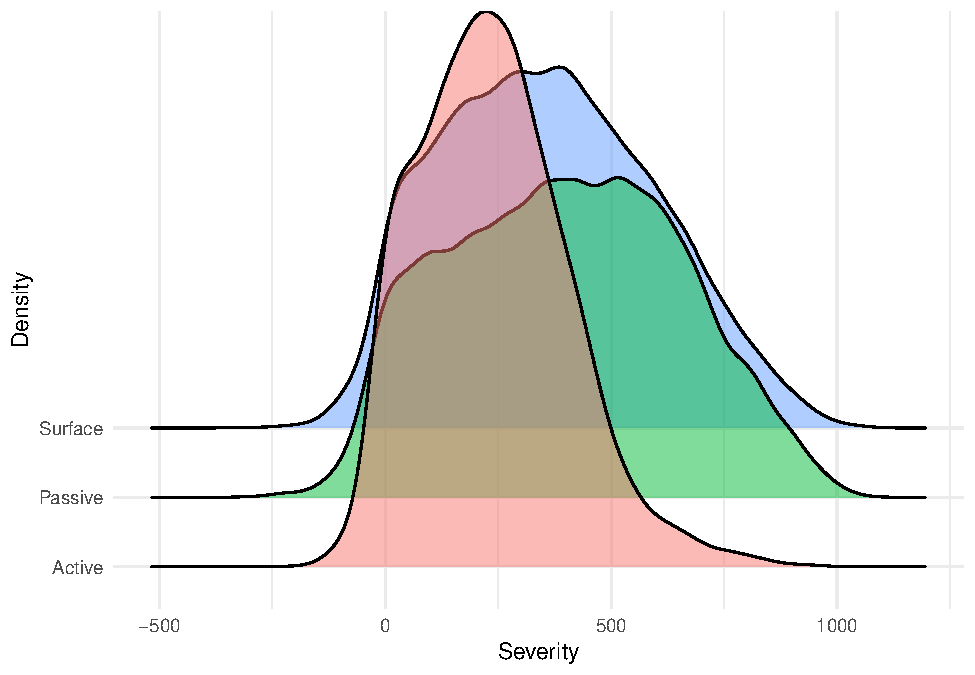
\includegraphics{term_project_files/figure-latex/fire_behavior-1.pdf}

Bar plot of canopy categories

\begin{Shaded}
\begin{Highlighting}[]
\NormalTok{forest_veg }\OperatorTok\StringTok{ }
\StringTok{  }\KeywordTok{left_join}\NormalTok{(severity, }\DataTypeTok{by =} \StringTok{"severity_id"}\NormalTok{) }\OperatorTok\StringTok{ }
\StringTok{  }\KeywordTok{filter}\NormalTok{(}\OperatorTok{!}\KeywordTok{is.na}\NormalTok{(severity_id)) }\OperatorTok\StringTok{ }
\StringTok{  }\KeywordTok{ggplot}\NormalTok{(}\KeywordTok{aes}\NormalTok{(}\DataTypeTok{x =}\NormalTok{ NVCSsubclass, }\DataTypeTok{y =}\NormalTok{ severity)) }\OperatorTok{+}
\StringTok{  }\KeywordTok{geom_boxplot}\NormalTok{() }\OperatorTok{+}
\StringTok{  }\KeywordTok{theme}\NormalTok{(}\DataTypeTok{axis.text.x =} \KeywordTok{element_text}\NormalTok{(}\DataTypeTok{angle =} \DecValTok{45}\NormalTok{, }\DataTypeTok{hjust =} \DecValTok{1}\NormalTok{)) }\OperatorTok{+}
\StringTok{  }\KeywordTok{labs}\NormalTok{(}\DataTypeTok{y =} \StringTok{"Severity (dNBR)"}\NormalTok{, }\DataTypeTok{x =} \StringTok{"Vegetation type"}\NormalTok{) }
\end{Highlighting}
\end{Shaded}

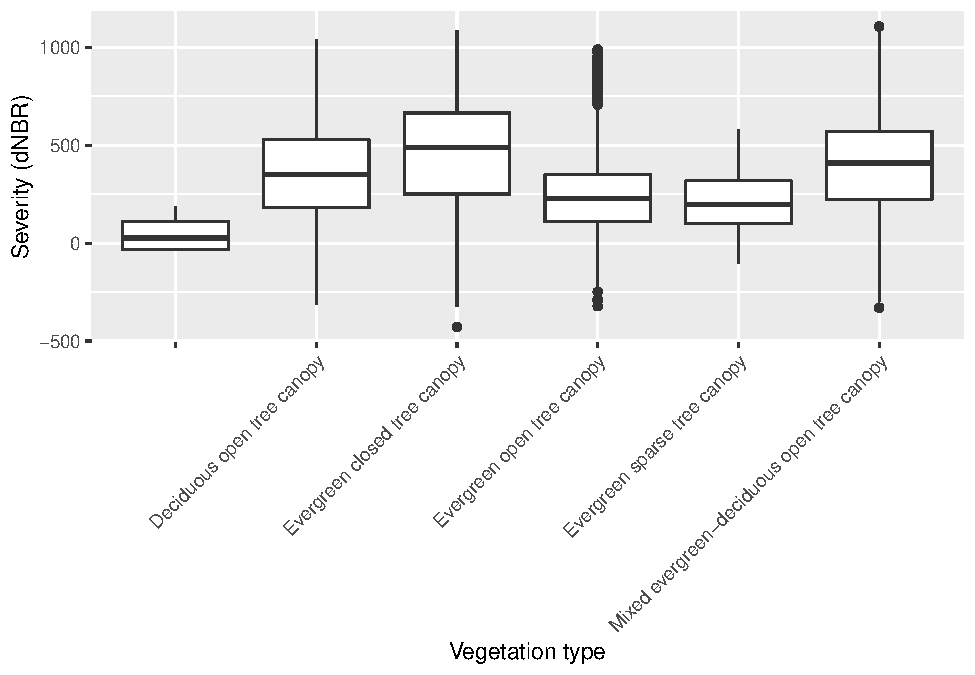
\includegraphics{term_project_files/figure-latex/fbarplot-1.pdf}

\bibliography{book.bib,packages.bib}

\end{document}
